\section{Эксперимент}

\tab Реакций тут не происходит, но при нагревании но происходящее 
описывется так. Не растворимы в обычных условиях $PbI_2$ при 
награвнии начинаект рассторятья. Потом расвор достигает 
максимальной концентации. Во время остывание весь растворившийся 
йодид свинца снова выпадат в виде осдка, но на этот раз в виде 
золотистых крислов.

\begin{figure}[h]
    \centering
    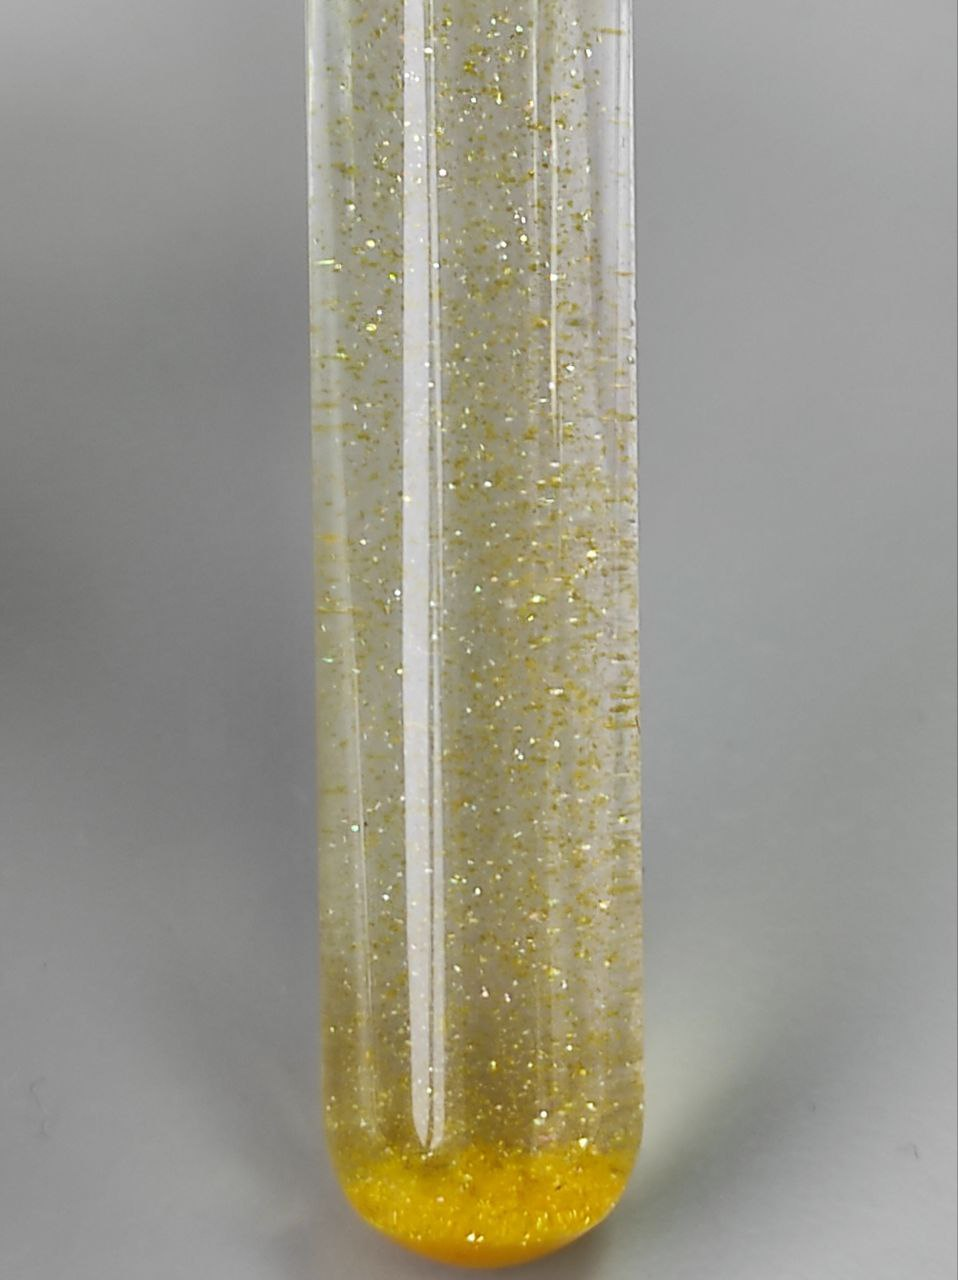
\includegraphics[width=0.6\linewidth]{Ex_7/crist.jpg}
     \caption{Кристализованный йодид свинца}
    \label{ex_7_1}
\end{figure}


